\subsection{Laplace Equation}
\subsubsection{Rectangular Domain}
The Laplace equation is of the form $$\nabla^2u=u_{xx}+u_{yy}=0$$
and is solved over a 2D domain. It is commonly the steady state of the heat or wave equation.\\
The solution method involves splitting the problem up into 4 subproblems with each subproblem having a solution similar to the wave equation.\\
\begin{center}
    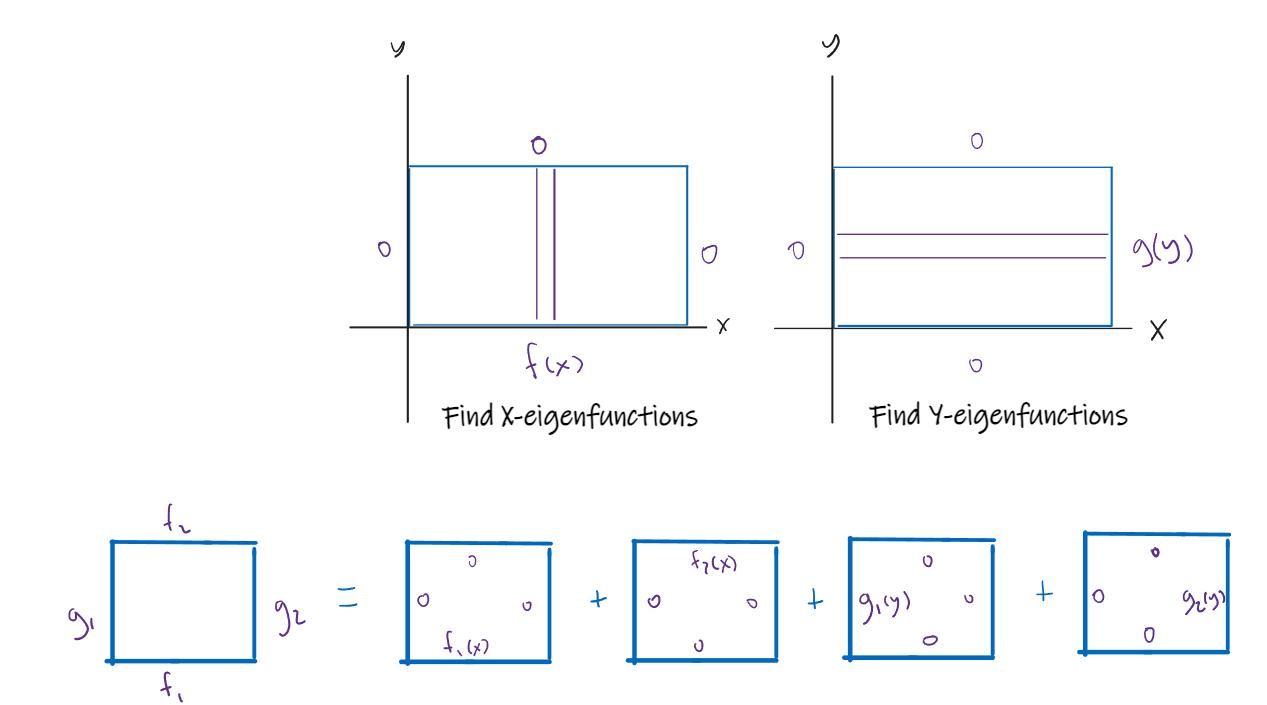
\includegraphics[width=14cm]{Images/PDEPictures/laplace.png}
\end{center}

\begin{enumerate}
    \item Draw out the domain and BCs
    \item Decompose into up to 4 subproblems
    \item Assume $u(x,y)=X(x)Y(y)$ so that $\frac{Y''}{Y}=\frac{-X''}{X}=\pm\lambda$
    \item Solve for eigenfunctions in the completely homogeneous axis first (see above). Here we cover the homogeneous $X$ case.
    \item Apply homogeneous boundary conditions to $X$ to fix $X_n$, $\lambda_n$ identical to eigenfunctions of heat equation boundary conditions.
    \item $Y_n$ will take the form of $Y_n(y) = A_n\cosh(\mu_n y)+B_n\sinh(\mu_ny)$
    \item Use the remaining homogeneous boundary to eliminate a coefficient or reduce the expression to $A_n=C \, B_n$ for some constant $C$ and rewrite the equation in terms of a single constant $Q_n$.  Using hyperbolic identities, the 8 common half-homogeneous boundary scenarios are listed below: 

\begin{tcolorbox}
\begin{center}
    \textbf{Common Laplace Equation Boundary Solutions}
\end{center}
\begin{multicols}{2}
If $u(x,0)=0$
\begin{align*}
    &u^{\text{top}}=\sum_{n=1}^\infty Q_n\sinh(\mu_n y)X_n
\end{align*}
If $u(x,b)=0$
\begin{align*}
    &u^{\text{bottom}}=\sum_{n=1}^\infty Q_n\sinh(\mu_n(y-b))X_n
\end{align*}
If $u(0,y)=0$
\begin{align*}
    &u^{\text{right}}=\sum_{n=1}^\infty Q_n\sinh(\mu_nx)Y_n
\end{align*}
If $u(a,y)=0$
\begin{align*}
    &u^{\text{left}}=\sum_{n=1}^\infty Q_n\sinh(\mu_n(x-a))Y_n
\end{align*}


If $u_y(x,0)=0$
\begin{align*}
    &u^{\text{top}}=\sum_{n=1}^\infty Q_n\cosh(\mu_n y)X_n
\end{align*}
If $u_y(x,b)=0$
\begin{align*}
    &u^{\text{bottom}}=\sum_{n=1}^\infty Q_n\cosh(\mu_n(y-b))X_n
\end{align*}
If $u_x(0,y)=0$
\begin{align*}
    &u^{\text{right}}=\sum_{n=1}^\infty Q_n\cosh(\mu_nx)Y_n
\end{align*}
If $u_x(a,y)=0$
\begin{align*}
    &u^{\text{left}}=\sum_{n=1}^\infty Q_n\cosh(\mu_n(x-a))Y_n
\end{align*}

\end{multicols}
\end{tcolorbox}

    \item Use the final in-homogenous boundary condition to find a Fourier relation to determine the coefficients $Q_n$
    
    \item Solve the remaining subproblems, the final solution is:
    $$u(x,y) = u(x,y)^{\text{left}} + u(x,y)^{\text{right}} + u(x,y)^{\text{top}} + u(x,y)^{\text{bottom}}$$
    * Some of the sub-problems have trivial solutions if there is no in-homogenous boundary condition for that side.

\end{enumerate}
\begin{align*}
    &u_{xx}+u_{yy}=0,\ 0\leq x\leq 3,\ 0\leq y\leq 2\\
    &u_x(0,y)=0.1,\ u_y(x,0)=0\\
    &u(x,2)=\eqnsystem{x & 0\leq x<1\\ 2-x & 1\leq x <3}\\
    &u(3,y)=\eqnsystem{y & 0\leq y<1\\ 2-y & 1\leq y <2}\\
    &u=u^A+u^B+u^C\\
    &u^A:\ u_x(0,y)\neq0\\
    &u^B:\ u(x,2)\neq0\\
    &u^C:\ u(3,y)\neq0
\end{align*}
Subproblem A:
\begin{align*}
    &u(x,y)=X(x)Y(y)\\
    &X''Y+XY''=0\Ra -\frac{X''}{X}=\frac{Y''}{Y}=-\lambda\\
    &u_y(x,0)=u(x,2)=0\\
    &\leadsto \lambda_n=\brround{\frac{2n-1}{2L}\pi}^2=\brround{\frac{2n-1}{4}\pi}^2\\
    &Y_n=\cos(\mu_n y),\ \mu_n=\frac{2n-1}{4}\pi\\
    &X_n=A_n\cosh(\mu_nx)+B_n\sinh(\mu_nx)\\
    &u(3,y)=0\Ra X(3)=0\\
    &A_n\cosh(3\mu_n)+B_n\sinh(3\mu_n)=0\Ra A_n=-B_n\frac{\sinh(3\mu_n)}{\cosh(3\mu_n)}\\
    &X_n=-B_n\frac{\sinh(3\mu_n)}{\cosh(3\mu_n)}\cosh(\mu_nx)+B_n\sinh(\mu_nx)\\
    &X_n=\frac{B_n}{\cosh(3\mu_n)}\brround{-\sinh(3\mu_n)\cosh(\mu_nx)+\sinh(\mu_nx)\cosh(3\mu_n)}\\
    &\sinh A\cosh B-\sinh B\cosh A=\sinh(A-B)\\
    &X_n=\frac{B_n}{\cosh(3\mu_n)}\sinh(\mu_n(x-3))\\
    &u^A=\sum_{n=1}^\infty Q_n\cos(\mu_n y)\sinh(\mu_n(x-3))\\
    &u_x^A=\sum_{n=1}^\infty Q_n\mu_n\cos(\mu_ny)\cosh(\mu_n(x-3))\\
    &u_x^A(0,y)=\sum_{n=1}^\infty \underbrace{Q_n\mu_n\cosh(-3\mu_n)}_{C_n}\sin(\mu_ny)=0.1\\
    &C_n=\frac{2}{2}\int_0^20.1\cos(\mu_ny)dy=\brsquare{0.1\frac{\sin{\mu_n y}}{\mu_n}}_0^2=\frac{0.1\sin(2\mu_n)}{\mu_n}\\
    &\sin(2\mu_n)=(-1)^{n+1}\\
    &Q_n=\frac{0.1(-1)^{n+1}}{\mu_n^2\cosh(-3\mu_n)}\\
    &u^A(x,y)=\sum_{n=1}^\infty\frac{0.1(-1)^{n+1}}{\mu_n^2\cosh(-3\mu_n)}\cos(\mu_ny)\sinh(\mu_n(x-3)),\ \mu_n=\frac{2n-1}{4}\pi
\end{align*}
Subproblem B:
\begin{align*}
    &\frac{X''}{X}=-\frac{Y''}{Y}=-\lambda\\
    &u_x(0,y)=u(3,y)=0\\
    &\leadsto\lambda_n=\brround{\frac{2n-1}{2L}\pi}^2=\brround{\frac{2n-1}{6}}^2\\
    &X_n=\cos(\mu_n x),\ \mu_n=\frac{2n-1}{6}\pi\\
    &Y_n=A_n\cosh(\mu_n y)+B_n\sinh(\mu_n y)\\
    &u_y(x,0)=0\Ra Y'(0)=0\\
    &Y_n'=A_n\mu_n\sinh(\mu_ny)+B_n\mu_n\cosh(\mu_ny)\\
    &Y'(0)=B_n\mu_n=0\Ra B_n=0\\
    &Y_n=A_n\cosh(\mu_ny)\\
    &u^B=\sum_{n=1}^\infty Q_n\cos(\mu_nx)\cosh(\mu_n y)\\
    &u^B(x,2)=\sum_{n=1}^\infty \underbrace{Q_n\cosh(2\mu_n)}_{C_n}\cos(\mu_nx)=\eqnsystem{x & 0\leq x<1\\ 2-x & 1\leq x <3}\\
    &C_n=\frac{2}{3}\int_0^1 x\cos(\mu_nx)dx+\frac{2}{3}\int_1^3(2-x)\cos(\mu_nx)dx\\
    &C_n=\frac{2\mu_n\sin(\mu_n)+2\cos(\mu_n)-2}{3\mu_n^2}+\frac{2\cos(\mu_n)-2\mu_n\sin(3\mu_n)-2\cos(3\mu_n)-2\mu_n\sin(\mu_n)}{3\mu_n^2}\\
    &\sin(3\mu_n)=(-1)^{n+1},\ \cos(3\mu_n)=0\\
    &C_n=\frac{4\cos(\mu_n)-2\mu_n(-1)^{n+1}-2}{3\mu_n^2}\\
    &Q_n=\frac{4\cos(\mu_n)-2\mu_n(-1)^{n+1}-2}{3\mu_n^2\cosh(2\mu_n)}\\
    &u^B=\sum_{n=1}^\infty\frac{4\cos(\mu_n)-2\mu_n(-1)^{n+1}-2}{3\mu_n^2\cosh(2\mu_n)}\cos(\mu_nx)\cosh(\mu_ny),\ \mu=\frac{2n-1}{6}\pi
\end{align*}
Subproblem C:
\begin{align*}
    &-\frac{X''}{X}=\frac{Y''}{Y}=-\lambda\\
    &u_y(x,0)=u(x,2)=0\\
    &\leadsto \lambda_n=\brround{\frac{2n-1}{2L}\pi}^2=\brround{\frac{2n-1}{4}\pi}^2\\
    &Y_n=\cos(\mu_n y),\ \mu_n=\frac{2n-1}{4}\pi\\
    &X_n=A_n\cosh(\mu_nx)+B_n\sinh(\mu_nx)\\
    &u_x(0,y)=0\Ra X'(0)=0\\
    &X'=A_n\mu_n\sinh(\mu_nx)+B_n\mu_n\cosh(\mu_nx)\\
    &X'(0)=B_n\mu_n=0\Ra B_n=0\\
    &X(x)=A_n\cosh(\mu_nx)\\
    &u^C=\sum_{n=1}^\infty Q_n\cos(\mu_n y)\cosh(\mu_n x)\\
    &u^C(3,y)=\sum_{n=1}^\infty \underbrace{Q_n\cosh(3\mu_n)}_{C_n}\cos(\mu_ny)=\eqnsystem{y & 0\leq y<1\\ 2-y & 1\leq y <2}\\
    &C_n=\frac{2}{2}\int_0^1y\cos(\mu_ny)dy+\frac{2}{2}\int_1^2(2-y)\cos(\mu_ny)dy\\
    &C_n=\frac{\mu_n\sin(\mu_n)+\cos(\mu_n)-1}{\mu_n^2}+\frac{\cos(\mu_n)-\cos(2\mu_n)-\mu_n\sin(\mu_n)}{\mu_n^2}=\frac{2\cos(\mu_n)-\cos(2\mu_n)-1}{\mu_n^2}\\
    &\cos(2\mu_n)=0\\
    &Q_n=\frac{2\cos(\mu_n)-1}{\mu_n^2\cosh(3\mu_n)}\\
    &u^C=\sum_{n=1}^\infty\frac{2\cos(\mu_n)-1}{\mu_n^2\cosh(3\mu_n)}\cos(\mu_ny)\cosh(\mu_nx),\ \mu_n=\frac{2n-1}{4}\pi
\end{align*}
Final solution:
\begin{align*}
    &u(x,y)=\sum_{n=1}^\infty\left(\brround{\frac{1.6(-1)^{n+1}\sinh\brround{\frac{2n-1}{4}\pi(x-3)}}{(2n-1)^2\pi^2\cosh(-3(\frac{2n-1}{4}\pi))}+\frac{16(2\cos(\frac{2n-1}{4}\pi)-1)\cosh(\frac{2n-1}{4}\pi x)}{(2n-1)^2\pi^2\cosh(3(\frac{2n-1}{4}\pi))}}\cos\brround{\frac{2n-1}{4}\pi y}\right.\\
    &\left.+\frac{24(\cos(\frac{2n-1}{6}\pi)-\frac{(2n-1)\pi(-1)^{n+1}}{6}-1)}{(2n-1)^2\pi^2\cosh(\frac{2n-1}{3}\pi)}\cos\brround{\frac{2n-1}{6}\pi x}\cosh\brround{\frac{2n-1}{6}\pi y}\right)
\end{align*}

\subsubsection{Circular Domain}
We can solve the Laplace equation on slightly more complicated domains. One very common one is circular domains.\\
To do this we will want to solve the Laplace equation in polar coordinates.
\begin{align*}
    &x=r\cos\theta,\ y=r\sin\theta\\
    &\nabla^2 u=u_{rr}+\frac{1}{r}u_r+\frac{1}{r^2}u_{\theta\theta}
\end{align*}
Using separation of variables we can get
\begin{align*}
    &u(r,\theta)=R(r)\Theta(\theta)\\
    &R''\Theta+\frac{1}{r}R'\Theta+\frac{1}{r^2}R\Theta''=0
\end{align*}
Multiply by $r^2$ and divide by $R\Theta$
\begin{align*}
    &-\brround{r^2\frac{R''}{R}+r\frac{R'}{R}}=\frac{\Theta''}{\Theta}=-\lambda
\end{align*}
We will have 2 different types of solutions:
\begin{enumerate}
    \item homogeneous boundary conditions in $\theta$
    \item homogeneous boundary conditions in $r$
\end{enumerate}
Along with the given boundary conditions, we also have the following implied boundary conditions:
\begin{itemize}
    \item If the domain contains $r=0$ then $\lim\limits_{r\to0}u(r,\theta)$ must be finite
    \item If the domain contains $r=\infty$ then $\lim\limits_{r\to\infty}u(r,\theta)$ must be finite
    \item If the domain forms a full circle/ring then the boundary conditions in $\theta$ are periodic
\end{itemize}
It is also important to note that you cannot use superposition on a circular domain like you can on a rectangular domain.\\
The general solution method for boundary value problems in $\theta$ is outlined below:
\begin{enumerate}
    \item The first thing to do is to make sure the boundary conditions in $\theta$ are homogeneous. If not then use the methods mentioned earlier to make them homogeneous.
    \item Solve the eigenvalue problem in $\Theta$ to get $\lambda_n$ and $\Theta_n$
    \item Plug in $\lambda_n$ and solve the ODE, $r^2R_n''+rR_n'-\lambda_n R_n=0$ to find $R_n$. The solution should be of the form ${R_n=A_nr^{\mu_n}+B_nr^{-\mu_n}}$
    \item Write out $u(r,\theta)=a_0\Theta_0R_0+\sum\limits_{n=1}^\infty\Theta_nR_n$ and impose the initial conditions in $r$ to solve for the unknown constants, $a_0,A_n,B_n$
\end{enumerate}
Ex: full circular domain with periodic BCs
\begin{align*}
    &u_{rr}+\frac{1}{r}u_\theta+\frac{1}{r^2}u_{\theta\theta}\\
    &u(a,\theta)=f(\theta),\ 0\leq r\leq a,\ -\pi\leq\theta\leq\pi
\end{align*}
This implies that the boundary conditions are
\begin{align*}
    &u(0,\theta)\text{ is finite}\\
    &u(a,\theta)=f(\theta)\\
    &u(r,\pi)=u(r,-\pi)\\
    &u_\theta(r,\pi)=u_\theta(r,-\pi)
\end{align*}
To solve, we will first solve the eigenvalue problem in $\theta$
\begin{align*}
    &-\brround{r^2\frac{R''}{R}+r\frac{R'}{R}}=\frac{\Theta''}{\Theta}=-\lambda\\
    &\Theta''+\lambda\Theta=0\\
    &\leadsto \lambda_0=0,\ \lambda_n=n^2,\ n\geq1\\
    &\Theta_0=1,\ \Theta_n=\eqnsystem{\cos(n\theta)\\\sin(n\theta)}
\end{align*}
For each $\lambda_n$, we can solve for $R_n$
\begin{align*}
    &\lambda_0:\\
    &r^2\frac{R_0''}{R_0}+r\frac{R_0'}{R_0}\Ra r^2R_0''+rR_0=0\\
    &\beta(\beta-1)+\beta=0\Ra \beta^2=0\\
    &R_0=C_0r^0+D_0\ln|r|r^0\\
    &R_0=C_0+D_0\ln r,\ 0<r\leq a\\
    &\lambda_n:\\
    &r^2\frac{R_n''}{R_n}+r\frac{R_n'}{R_n}=n^2\Ra r^2R_n''+rR_n'-n^2R_n\\
    &\beta(\beta-1)+\beta-n^2=0\Ra \beta^2=n^2\Ra \beta=\pm n\\
    &R_n=C_nr^n+D_nr^{-n}\\
    &\lim_{r\to0} R_0(r)\neq\pm\infty\Ra \lim_{r\to0}\brround{C_0+D_0\ln r}\neq\pm\infty\Ra D_0=0\Ra R_0=1\\
    &\lim_{r\to0} R_n(r)\neq\pm\infty\Ra \lim_{r\to0}\brround{C_nr^n+D_nr^{-n}}\neq\pm\infty\Ra D_n=0\Ra R_n=r^n
\end{align*}
Now that we have $R$ and $\Theta$ we can put them together to get
\begin{align*}
    &u(r,\theta)=C_0+\sum_{n=1}^\infty r^n\brround{C_n\cos(n\theta)+D_n\sin(n\theta)}\\
    &u(a,\theta)=f(\theta)=C_0+\sum_{n=1}^\infty a^nC_n\cos(n\theta)+a^nD_n\sin(n\theta)\\
    &C_0=\frac{1}{2\pi}\int_{-\pi}^\pi f(\theta)d\theta\\
    &C_n=\frac{1}{\pi a^n}\int_{-\pi}^\pi f(\theta)\cos(n\theta)d\theta\\
    &D_n=\frac{1}{\pi a^n}\int_{-\pi}^\pi f(\theta)\sin(n\theta)d\theta
\end{align*}
Ex2:
\begin{align*}
    &0<a\leq r\leq b,\ 0\leq\theta\leq\frac{\pi}{2}\\
    &u_{rr}+\frac{1}{r}u_r+\frac{1}{r^2}u_{\theta\theta}\\
    &u_\theta(r,0)=0,\ u\brround{r,\frac{\pi}{2}}=2\\
    &u(a,\theta)=\cos(2\theta),\ u(b,\theta)=0\\
    &u^A:\ v\brround{r,\frac{\pi}{2}}\neq 0\\
    &u^B:\ v(a,\theta)\neq 0
\end{align*}
Steady State:
\begin{align*}
    &u(r,\theta)=w(\theta)+v(r,\theta)\\
    &\nabla^2w=0\Ra w(\theta)=A\theta+B\\
    &w'(0)=0\Ra A=0\\
    &w\brround{\frac{\pi}{2}}=2=B\\
    &w(\theta)=2\\
    &\nabla^2u=\nabla^2 v\\
    &u_\theta(r,0)=w_\theta(0)+v_\theta(r,0)=0\Ra v_\theta(r,0)=0\\
    &u\brround{r,\frac{\pi}{2}}=w\brround{\frac{\pi}{2}}+v\brround{r,\frac{\pi}{2}}\Ra v\brround{r,\frac{\pi}{2}}\\
    &u(a,\theta)=w(\theta)+v(a,\theta)=2+v(a,\theta)=\cos(2\theta)\Ra v(a,\theta)=\cos(2\theta)-2\\
    &u(b,\theta)=w(\theta)+v(b,\theta)=0\Ra v(b,\theta)=-2
\end{align*}
Eigenvalue problem:
\begin{align*}
    &v_\theta(r,0)=0,\ v\brround{r,\frac{\pi}{2}}=0\\
    &-\brround{r^2\frac{R''}{R}+r\frac{R'}{R}}=\frac{\Theta''}{\Theta}=-\lambda\\
    &\leadsto\lambda_n=\brround{\frac{2n-1}{2L}\pi}^2=\brround{2n-1}^2\\
    &\Theta_n=\cos(\mu_n\theta),\ \mu_n=2n-1\\
    &r^2R_n''+rR_n'-\mu_n^2R_n=0\\
    &\beta(\beta-1)+\beta-\mu_n^2=\beta^2-\mu_n^2=0\Ra \beta=\pm\mu_n\\
    &R_n=A_nr^{\mu_n}+B_nr^{-\mu_n}\\
    &v(r,\theta)=\sum_{n=1}^\infty(A_nr^{\mu_n}+B_nr^{-\mu_n})\cos(\mu_n\theta)\\
    &v(b,\theta)=\sum_{n=1}^\infty\underbrace{(A_nb^{\mu_n}+B_nb^{-\mu_n})}_{C_n}\cos(\mu_n\theta)=-2\\
    &C_n=\frac{4}{\pi}\int_0^{\pi/2}-2\cos(\mu_n\theta)d\theta=\frac{-8}{\mu_n\pi}\sin(\mu_n\theta)\eval_0^{\pi/2}=\frac{8(-1)^n}{\mu_n\pi}\\
    &v(a,\theta)=\sum_{n=1}^\infty\underbrace{(A_na^{\mu_n}+B_na^{-\mu_n})}_{D_n}\cos(\mu_n\theta)=\cos(2\theta)-2\\
    &D_n=\frac{4}{\pi}\int_0^{\pi/2}(\cos(2\theta)-2)\cos(\mu_n\theta)d\theta=C_n+\frac{4}{\pi}\int_0^{\pi/2}\cos(2\theta)\cos(\mu_n\theta)d\theta\\
    &D_n=C_n+\frac{4}{\pi}\brround{\frac{(\mu_n-2)\sin(\frac{\mu_n+2}{2}\pi)+(\mu_n+2)\sin(\frac{\mu_n-2}{2}\pi))}{2(\mu_n^2-4)}}=C_n+\underbrace{\frac{4\mu_n(-1)^n}{(\mu_n^2-4)\pi}}_{K_n}\\
    &\eqnsystem{A_nb^{\mu_n}+B_nb^{-\mu_n}=C_n\\ A_na^{\mu_n}+B_na^{-\mu_n}=C_n}\Ra \matrixx{b^{\mu_n} & b^{-\mu_n}\\ a^{\mu_n} & a^{-\mu_n}}\matrixx{A_n\\B_n}=\matrixx{C_n\\D_n}\\
    &\matrixx{A_n\\B_n}=\frac{1}{(\frac{b}{a})^{\mu_n}-(\frac{a}{b})^{\mu_n}}\matrixx{a^{-\mu_n} & -b^{-\mu_n}\\ -a^{\mu_n} & b^{\mu_n}}\matrixx{C_n\\D_n}=\frac{1}{(\frac{b}{a})^{\mu_n}-(\frac{a}{b})^{\mu_n}}\matrixx{(a^{-\mu_n}-b^{-\mu_n})C_n\\ (b^{\mu_n}-a^{\mu_n})D_n}
\end{align*}
\begin{align*}
    &u(r,\theta)=2+\sum_{n=1}^\infty\left(\frac{8(-1)^n((a^{-(2n-1)}-b^{-(2n-1)})r^{(2n-1)}+(b^{(2n-1)}-a^{(2n-1)})r^{-(2n-1)})}{((\frac{b}{a})^{(2n-1)}-(\frac{a}{b})^{(2n-1)})(2n-1)\pi}\right.\\
    &\left.+\frac{\frac{4(2n-1)(-1)^n}{((2n-1)^2-4)\pi}(b^{(2n-1)}-a^{(2n-1)})r^{-(2n-1)}}{(\frac{b}{a})^{(2n-1)}-(\frac{a}{b})^{(2n-1)}}\right)\cos((2n-1)\theta)
\end{align*}